\documentclass[10pt]{article}
\usepackage{mathtools}
\usepackage{tikz}
\usepackage{verbatim}
\usepackage[left=2cm, right=2cm, top=1cm, bottom=2cm]{geometry}
\title {Mathematics 220 Calculus II, Homework \#1}
\author{Aleksander Charatonik}
\date{September 4, 2018}
\begin{document}
\maketitle
\section{}
First, we should draw the functions \(y=\sqrt{x}\), \(y=0\), and \(x=9\), so we can visualize the area we are working with, as well as the line \(y=5\) so we know what we are rotating about.\\
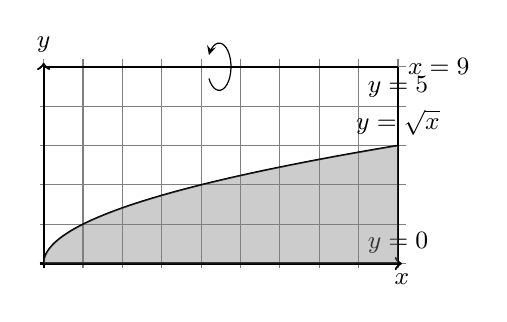
\begin{tikzpicture}[domain=0:9, scale=0.5]
  \newcommand{\AxisRotator}[1][rotate=0]{%
    \tikz [x=0.15cm,y=0.30cm,line width=.2ex,-stealth,#1] \draw (0,0) arc (-150:150:1 and 1);%
  }
  \draw[thin, gray](-0.1, -0.1) grid (9.2, 5.2);
  \draw[thick] [->] (-0.1,0)--(9.1,0) node[right, below] {\small \(x\)};
  \draw[thick] [->] (0,-0.1)--(0,5.1) node[left, above] {\small \(y\)};
  \draw[semithick, smooth, variable=\x, samples=500] plot[id=sqrtx] ({\x},{sqrt(\x)}) node[right, above] {\small \(y=\sqrt{x}\)};
  \draw[semithick, variable=\x] plot[id=y0] ({\x},{0}) node[left, above] {\small \(y=0\)};
  \draw[semithick, variable=\y,domain=0:5] plot[id=x9] ({9},{\y}) node[right] {\small \(x=9\)};
  \draw[semithick, variable=\x] plot[id=y5] ({\x}, {5}) node[below] {\small \(y=5\)};
  \draw[semithick] (4.5,5) node {\tiny \AxisRotator};
  \filldraw[
    fill=gray,
    samples=500,
    opacity=0.4
  ]
    plot[domain=0:9]
      (\x, {sqrt(\x)})
     -- (9,0) -- cycle;
\end{tikzpicture}\\

Here, we will use the washer method, with the outer radius being the distance of the X axis from \(y=5\), and the inner radius, the distance of \(\sqrt{x}\) from \(y=5\). We can take a slice of the graph, at some \(x\), with a thickness of \(\Delta x\). \\
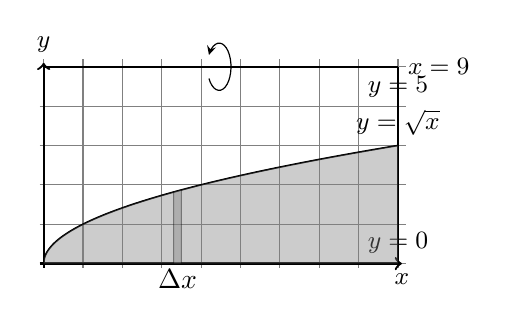
\begin{tikzpicture}[domain=0:9, scale=0.5]
  \newcommand{\AxisRotator}[1][rotate=0]{%
    \tikz [x=0.15cm,y=0.30cm,line width=.2ex,-stealth,#1] \draw (0,0) arc (-150:150:1 and 1);%
  }
  \draw[thin, gray](-0.1, -0.1) grid (9.2, 5.2);
  \draw[thick] [->] (-0.1,0)--(9.1,0) node[right, below] {\small \(x\)};
  \draw[thick] [->] (0,-0.1)--(0,5.1) node[left, above] {\small \(y\)};
  \draw[semithick, smooth, variable=\x, samples=500] plot[id=sqrtx] ({\x},{sqrt(\x)}) node[right, above] {\small \(y=\sqrt{x}\)};
  \draw[semithick, variable=\x] plot[id=y0] ({\x},{0}) node[left, above] {\small \(y=0\)};
  \draw[semithick, variable=\y,domain=0:5] plot[id=x9] ({9},{\y}) node[right] {\small \(x=9\)};
  \draw[semithick, variable=\x] plot[id=y5] ({\x}, {5}) node[below] {\small \(y=5\)};
  \draw[semithick] (4.5,5) node {\tiny \AxisRotator};
  \filldraw[
    fill=gray,
    samples=500,
    opacity=0.4
  ]
    plot[domain=0:9]
      (\x, {sqrt(\x)})
     -- (9,0) -- cycle;
  \filldraw[
    fill=gray,
    samples=500,
    opacity=0.4
  ]
    plot[domain=3.3:3.5]
      (\x, {sqrt(\x)})
     -- (3.5,0) -- (3.3,0) -- cycle;
  \draw (3.4, -0.4) node {\(\Delta x\)};
\end{tikzpicture}\\
The area of this rectangle is clearly \(\Delta x (9-\sqrt{x})\). And the volume generated by rotating that rectangle would be \(\pi \Delta x (9^2-\sqrt{x}^2)\). And of course, the summation of those rectangles, as they become thinner and thinner and approxomate reality is the integral. So we get \(\pi\int\limits_0^9 (81-x)dx\). Which becomes \(\pi(81x-\frac{x^2}{2}) |_0^9\), and evaluates to \(\pi (729-\frac{81}{2})\).\\

\section{}
Similarly to the first problem, we first draw the function, and note relevant information like the axis of rotation, and choose a slice at location \(x\), with thickness \(\Delta X\).\\
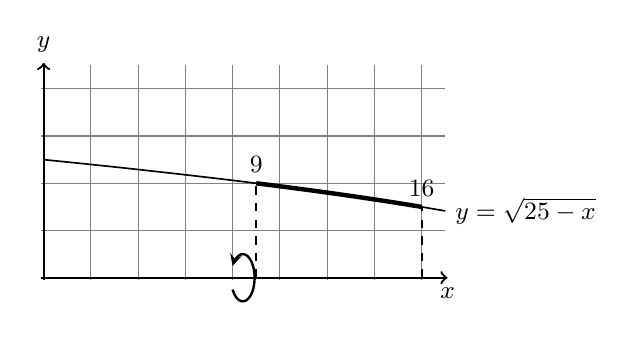
\begin{tikzpicture}[domain=0:17, scale=0.3]
  \newcommand{\AxisRotator}[1][rotate=0]{%
    \tikz [x=0.15cm,y=0.30cm,line width=.2ex,-stealth,#1] \draw (0,0) arc (-150:150:1 and 1);%
  }
  \draw[thin, gray, step=2](-0.1, -0.1) grid (17, 9);
  \draw[thick] [->] (-0.1,0)--(17.1,0) node[right, below] {\small \(x\)};
  \draw[thick] [->] (0,-0.1)--(0,9.1) node[left, above] {\small \(y\)};
  \draw[semithick, variable=\x] plot[id=sqrt25-x] ({\x},{sqrt(25-\x)}) node[right] {\small \(y=\sqrt{25-x}\)};
  \draw (8.5, 0) node {\AxisRotator};
  \draw[ultra thick, variable=\x, domain=9:16] plot[id=range] ({\x},{sqrt(25-\x)});
  \draw[thick, dashed] (9,0)--(9,4) node[above] {\small \(9\)};
  \draw[thick, dashed] (16,0)--(16,3) node[above] {\small \(16\)};

\end{tikzpicture}\\
Instead of approximating the area underneath with a rectangle, we're approximating the length with a straight line. We can pick an arbitrary point at \(x\), with a length \(\Delta x\). We can find that line easily once we notice that the top of that area forms a triangle.\\
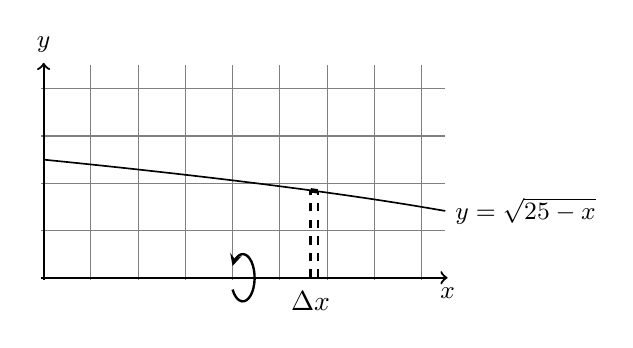
\begin{tikzpicture}[domain=0:17, scale=0.3]
  \newcommand{\AxisRotator}[1][rotate=0]{%
    \tikz [x=0.15cm,y=0.30cm,line width=.2ex,-stealth,#1] \draw (0,0) arc (-150:150:1 and 1);%
  }
  \draw[thin, gray, step=2](-0.1, -0.1) grid (17, 9);
  \draw[thick] [->] (-0.1,0)--(17.1,0) node[right, below] {\small \(x\)};
  \draw[thick] [->] (0,-0.1)--(0,9.1) node[left, above] {\small \(y\)};
  \draw[semithick, variable=\x] plot[id=sqrt25-x] ({\x},{sqrt(25-\x)}) node[right] {\small \(y=\sqrt{25-x}\)};
  \draw (8.5, 0) node {\AxisRotator};
  \draw[ultra thick, variable=\x, domain=11.3:11.6] plot[id=range] ({\x},{sqrt(25-\x)});
  \draw[thick, dashed] (11.3,0)--(11.3,3.7);
  \draw[thick, dashed] (11.6,0)--(11.6,3.66);
  \draw (11.3, -1) node {\(\Delta x\)};

\end{tikzpicture}
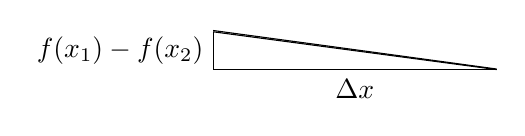
\begin{tikzpicture}[domain=11.3:11.6, scale=12]
  \draw plot ({\x},{sqrt(25-\x)});
  \draw (11.3,3.7)--(11.6,3.66);
  \draw (11.3,3.66)--(11.6,3.66) node[midway, below] {\(\Delta x\)};
  \draw (11.3,3.66)--(11.3,3.7) node[left, midway] {\(f(x_1)-f(x_2)\)};
\end{tikzpicture}\\
And by the pythagorean theorem, we can easily see that the length of the long side is \(\sqrt{\Delta x^2+(f(x_1)-f(x_2))^2}\). By the mean value theorem, we know that there is a point such that \(f'(x^{*}) \Delta x = (f(x_1)-f(x_2))\). We get, then \(\sqrt{\Delta x^2+[f'(x)]^2\Delta x^2}\), which is the same as \(\sqrt{(1+[f'(x)]^2)}\Delta x\), which we can take that infinite sum of, resulting in the integral. \(\int\sqrt{1+[f'(x)]^2}dx\).\\
Let's quickly find \((y')^2\). Using the chain rule, \(y'\) is \(-\frac{1}{2}\frac{1}{\sqrt{25-x}}\), and the square of that is \(\frac{1}{4}\frac{1}{25-x}\).

Now, let's finally, using the length we've found, let's finally see what the area is. The formula for the surface area of a frustum is simple. \(A=\pi(r_1+r_2)l\), where \(r_1\) and \(r_2\) are the radii of the two ends, and \(l\) is the length of the frustum. Substitute in the correct values, add the infinite sum, and we get our integral, which we can now evaluate.\\
\(2\pi\int_9^{16}\sqrt{25-x}\sqrt{1+\frac{1}{100-4x}}dx\)\\
With u substitution, \(u=25-x, du=-dx\). In our integral, replace 9 with a 16, and 16 with a 9, and we get \(-2\pi\int_{16}^9\sqrt{u}\sqrt{1+\frac{1}{4u}}du\), which in turn can be factored into \(-2\pi\int_{16}^9\frac{1}{2}\sqrt{4u+1}du\). Substitute again, \(v=4u+1, dv=4du, \frac{1}{4}dv=du\), correct the integral, 16 becomes 65, 9 becomes 37, for a final integral of \(-2\pi\int_{65}^{37}\frac{1}{2}\sqrt{v}\).\\

\(-\pi(\frac{2}{3}v^{\frac{3}{2}})|_{65}^{37}=-\pi(\frac{2}{3}37^{\frac{3}{2}}-\frac{2}{3}65^{\frac{3}{2}})\).

\section{}
Once again, begin by drawing a graph.\\ 
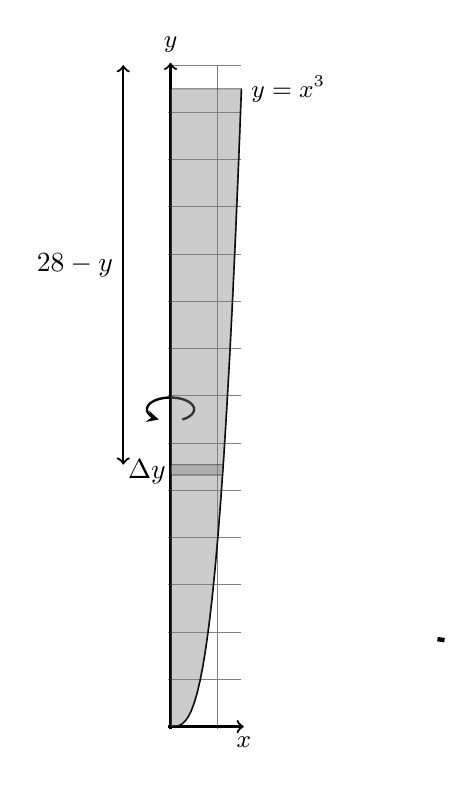
\begin{tikzpicture}[domain=0:3, scale=0.3]
  \newcommand{\AxisRotator}[1][rotate=0]{%
    \tikz [x=0.15cm,y=0.30cm,line width=.2ex,-stealth,#1] \draw (0,0) arc (-150:150:1 and 1);%
  }
  \draw[thin, gray, step=2](-0.1, -0.1) grid (3, 28);
  \draw[thick] [->] (-0.1,0)--(3.1,0) node[right, below] {\small \(x\)};
  \draw[thick] [->] (0,-0.1)--(0,28.1) node[left, above] {\small \(y\)};
  \draw[semithick, variable=\x] plot[id=sqrt25-x] ({\x},{\x^3}) node[right] {\small \(y=x^3\)};
  \draw (0, 13.5) node {\AxisRotator[rotate=90]};
  \draw[ultra thick, variable=\x, domain=11.3:11.6] plot[id=range] ({\x},{sqrt(25-\x)});
  \filldraw[
    fill=gray,
    samples=500,
    opacity=0.4
  ]
    plot[domain=0:3]
      (\x, {\x^3})
     -- (0,27) -- cycle;
  \filldraw[
    fill=gray,
    samples=500,
    opacity=0.4
  ]
    plot[domain=2.2:2.23]
      (\x, {\x^3)})
     -- (0,11.09) -- (0,10.648) -- cycle;
  \draw (-1, 10.8) node {\(\Delta y\)};
  \draw[thick] [<->] (-2,11.09)--(-2,28) node[midway, left] {\(28-y\)};


\end{tikzpicture}

Now, as we are rotating around the y axis, we want x in terms of y. This is simply \(x=\sqrt[3]{y}\). Next, we want to find a formula for the volume of liquid at a height \(y\). Since we can simply imagine this as a cylinder of height \(\Delta y\), this is simply \(\pi\sqrt[3]{y}^2\Delta y\). Weight is simply volume\(*\)density, and the work required to push 1 meter above the surface is the weight times the remaining distance. The total distance being \(3^3+1\), so \((28-y)*\rho*V\).\\
Take the infinite sum, and plug everything in, and we get our integral.\\ \(30kg/m^3\pi\int_{0m}^{27m}(28-y)\sqrt[3]{y}^2dy = 30kg/m^3\pi\int_{0m}^{27m}(28y^{\frac{2}{3}}-y^{\frac{4}{3}})dy\)\\
Evaluate:\\
\(30kg/m^3\pi(\frac{84}{5}y^{\frac{5}{3}}-\frac{3}{7}y^{\frac{7}{3}})|_{0m}^{27m} = 30kg/m^3\pi(\frac{20412}{5}m^{\frac{5}{3}}-\frac{6561}{7}m^{\frac{7}{3}}) = 30\pi(\frac{20412}{5}-\frac{6561}{7})J\).

\section{}
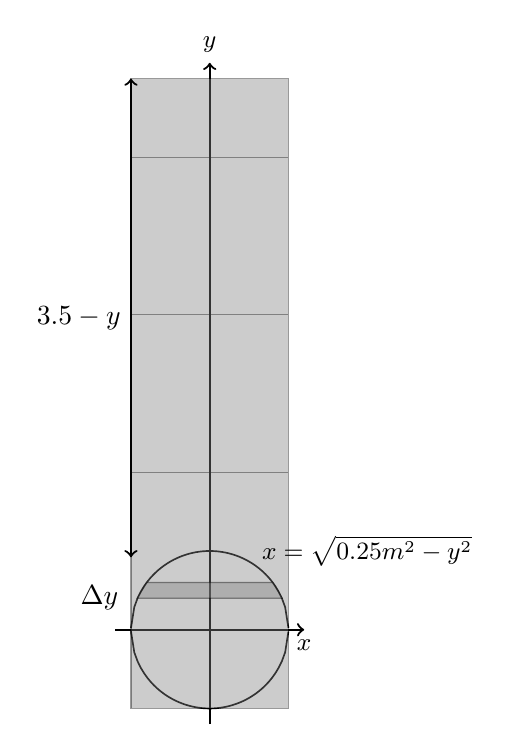
\begin{tikzpicture}[domain=-0.5:3.5, scale=2]
  \newcommand{\AxisRotator}[1][rotate=0]{%
    \tikz [x=0.15cm,y=0.30cm,line width=.2ex,-stealth,#1] \draw (0,0) arc (-150:150:1 and 1);%
  }
  \draw[thin, gray, step=1](-0.5, -0.5) grid (0.5, 3.5);
  \draw[thick] [->] (-0.6,0)--(0.6,0) node[right, below] {\small \(x\)};
  \draw[thick] [->] (0,-0.6)--(0,3.6) node[left, above] {\small \(y\)};
  \draw[semithick, variable=\x, domain=0:0.5] plot[id=sqrt25-x] ({\x},{sqrt(0.25-\x^2)}) ;
  \draw[semithick, variable=\x, domain=-0.4999:0] plot[id=sqrt25-x] ({\x},{sqrt((\x^2)+0.25)});
  \draw[semithick, variable=\x, domain=0:0.5] plot[id=sqrt25-x] ({\x},{-sqrt(0.25-\x^2)});
  \draw[semithick, variable=\x, domain=-0.4999:0] plot[id=sqrt25-x] ({\x},{-sqrt((\x^2)+0.25)});
  \node (a) at (-0.4,0.3) {};
  \node (b) at (0.4,0.3) {};
  \node (c) at (0.46,0.2) {};
  \node (d) at (-0.46,0.2) {};
  \filldraw[
    fill=gray,
    samples=500,
    opacity=0.4
  ]
      (-0.5,-0.5) -- (0.5,-0.5)
     -- (0.5,3.5) -- (-0.5,3.5) -- cycle;
  \filldraw[
    fill=gray,
    samples=500,
    opacity=0.4
  ]
      (a.center)--(b.center)--(c.center)--(d.center)--cycle;
  \draw (-0.7,0.2) node {\(\Delta y\)};
  \draw[thick] [<->] (-0.5,0.46)--(-0.5,3.5) node[midway, left] {\(3.5-y\)};
  \draw (1,0.5) node {\small \(x=\sqrt{0.25m^2-y^2}\)};
\end{tikzpicture}


The hydrostatic pressure at a given depth is simply \(\rho g d\), where \(\rho\) is the density, g is the force of gravity, and d is the depth. The hydrostatic force on an area A is the pressure times A.\\
The equation for the circle at a given point x is simply \(2\sqrt{r^2-y^2}\).
If we place the coordinate system at the center of the window, for simplycity's sake, then the top of the water is at \(y=3.5\). The pressure at any given depth \(y\) then is \((3.5-y)\rho g\). The area of a strip, of height \(\Delta y\) and depth \(y\) is just \(2\sqrt{0.25m^2-ym^2}\Delta y\). The hydrostatic force is the limit of all these thin strips, so we get:\\
2\(\rho g\int_{-0.5m}^{0.5m}(3.5-y)\sqrt{0.25m^2-y^2}dy\), which we split into two integrals:\\
\(2\rho g(\int_{-0.5m}^{0.5m}3.5\sqrt{0.25m^2-y^2}dy-\int_{-0.5m}^{0.5m}y\sqrt{0.25m^2-y^2}dy)\).\\
For the first integral, take out the \(\frac{1}{4}\), so we get a \(\int_{-0.5m}^{0.5m}1.75\sqrt{1m^2-4y^2}dy\). Apply trig substitution, \(y=\frac{1}{2}sin(u)\). \(1.75\int_{-\frac{\pi}{6}}^{\frac{\pi}{6}}\frac{1}{2}cos^2(u)du\).\\
For the second integral, \(u=y^2, du=2y\), replace the -0.5m and 0.5m both with 0.25m, which evaluates to zero. So now all that's left is to evaluate the first integral:\\
\(3.5\rho g\int_{-\frac{\pi}{6}}^{\frac{\pi}{6}}\frac{1}{2}cos^2(u)du = 3.5\rho g(\frac{1}{4}(x+sin(x)cos(x)))|_{-\frac{\pi}{6}}^{\frac{\pi}{6}} =\\
3.5\rho g(\frac{1}{4}(\frac{\pi}{6}+\frac{\sqrt{3}}{4}+\frac{\pi}{6}+\frac{\sqrt{3}}{4}))\).

\end{document}
